\documentclass{jarticle}

\usepackage{twocolumn}
% \usepackage[dvi ps]{graphicx}%%画像を読み込む
\usepackage[dvipdfmx]{graphicx}
\usepackage{subfigure}
\usepackage{amsmath}          %%genfrac http://www.biwako.shiga-u.ac.jp/sensei/kumazawa/tex/form006.html
\usepackage{ulem}             %%http://biwako.shiga-u.ac.jp/sensei/kumazawa/tex/ulem.html     uline,uuline,uwave,sout,xoutなど
\usepackage{multirow}
% \usepackage{setspace}
\usepackage{chukan2018}       %%最後に読み込むこと!(最後に読み込まないと\textwidthなどの設定が反映されない)

\pagestyle{empty} %ページ番号を入れるときにはコメントアウトする

\begin{document}

\linesparpage{50}

\title{
細径空圧筋を用いた外骨格生物模倣ロボットの開発
}
\etitle{
Development of an Exoskeletal Biomimetic Robot Using Fine Pneumatic Muscles
}
\author{
研究者 濱口 紘生  指導教員  中西 大輔
}
\eauthor{
Keywords: McKibben Pneumatic Actuater, Exoskeleton, Biomimetic Robot
}

\maketitle

\thispagestyle{empty}  %1ページ目にページ番号を入れるときにはコメントアウトする

%%%%%%%%%%%%%%%%%%%%%%%%%%%%%%%%%%%%%%%%%%%%%%%%%%%%%%%%%%%%%%%%%%%%%%%%%%%%%%%
\section{緒言}

代表的な人工筋肉として,圧縮空気を印加することにより骨格筋のように収縮するMcKibben型人工筋肉(MPA)
があげられる.従来は直径が数十mm程度のものが多かったが,近年では数mm程度のMPAが注目を集めている\cite{wakimoto}.
その細さを生かして小さい筋肉,あるいは集積によって単純な紡錘形以外の筋肉を表現可能なことから,筋骨格系ロボットにおいて特盛んに用いられている\cite{wakimoto}.
一方で,甲殻類をはじめとする外骨格を有する生物模倣ロボットについては,ワイヤ駆動や関節にサーボモータを配置したものが主流であった\cite{crabrobot}.
これは外骨格内部にアクチュエータを配置するのが困難なためである.
細径MPAであれば骨格内部にアクチュエータを配置することが可能であり,実際の生物に近い構成でロボットを作成することが可能である.
そこで本研究では外骨格生物のうち甲殻類の蟹をモデルに,実際の蟹の筋肉と関節の構造を参考にして細径MPAを使用した蟹の歩脚ロボットの開発に取り組む.

%%%%%%%%%%%%%%%%%%%%%%%%%%%%%%%%%%%%%%%%%%%%%%%%%%%%%%%%%%%%%%%%%%%%%%%%%%%%%%%
\vspace*{-2mm}
\section{MPAおよび生物モデルについて}

\vspace*{-1mm}
\subsection{細径MPAについて}

従来のMPAと細径MPAを図~に示す.細径MPAの特徴として以下の点が挙げられる.1つ目に細くて軽量のため限られた狭いスペースへの配置と集積が可能,2つ目に集積化により収縮量増大させること,
3つ目に集積化により羽状筋のような複雑な筋肉の再現が可能であること.

%%%%%%%%%%%%%%%%%%%%%%%%%%%%%%%%%%%%%%%%%%%%%%%%%%%%%%%%%%%%%%%%%%%%%%%%%%%%%%%
\vspace*{-1mm}
\subsection{外骨格生物のモデルについて}

蟹などの甲殻類の脚は鋏脚と歩脚の5対10本からなる.
脚は7つの節から構成されており,それぞれ甲に近いほうから,底節,基節,座節,長節,腕節,前節,指節と呼ばれている\cite{crab}.
長節以降の節は直交しており,手先は3次元運動することが可能である.
また,甲殻内部は図~のように筋肉と腱と呼ばれる組織で構成されている.
筋繊維の一端は甲殻の内壁に付着し,もう一方は腱に付着することによって各節を繋げ脚を開閉させている.
なお底節,基節,座節部分は筋配置が複雑なため省略し,本研究では長節以降の歩脚の再現を目指す.



\begin{figure}[t]
  \begin{minipage}[b]{0.47\columnwidth}
    \centering
    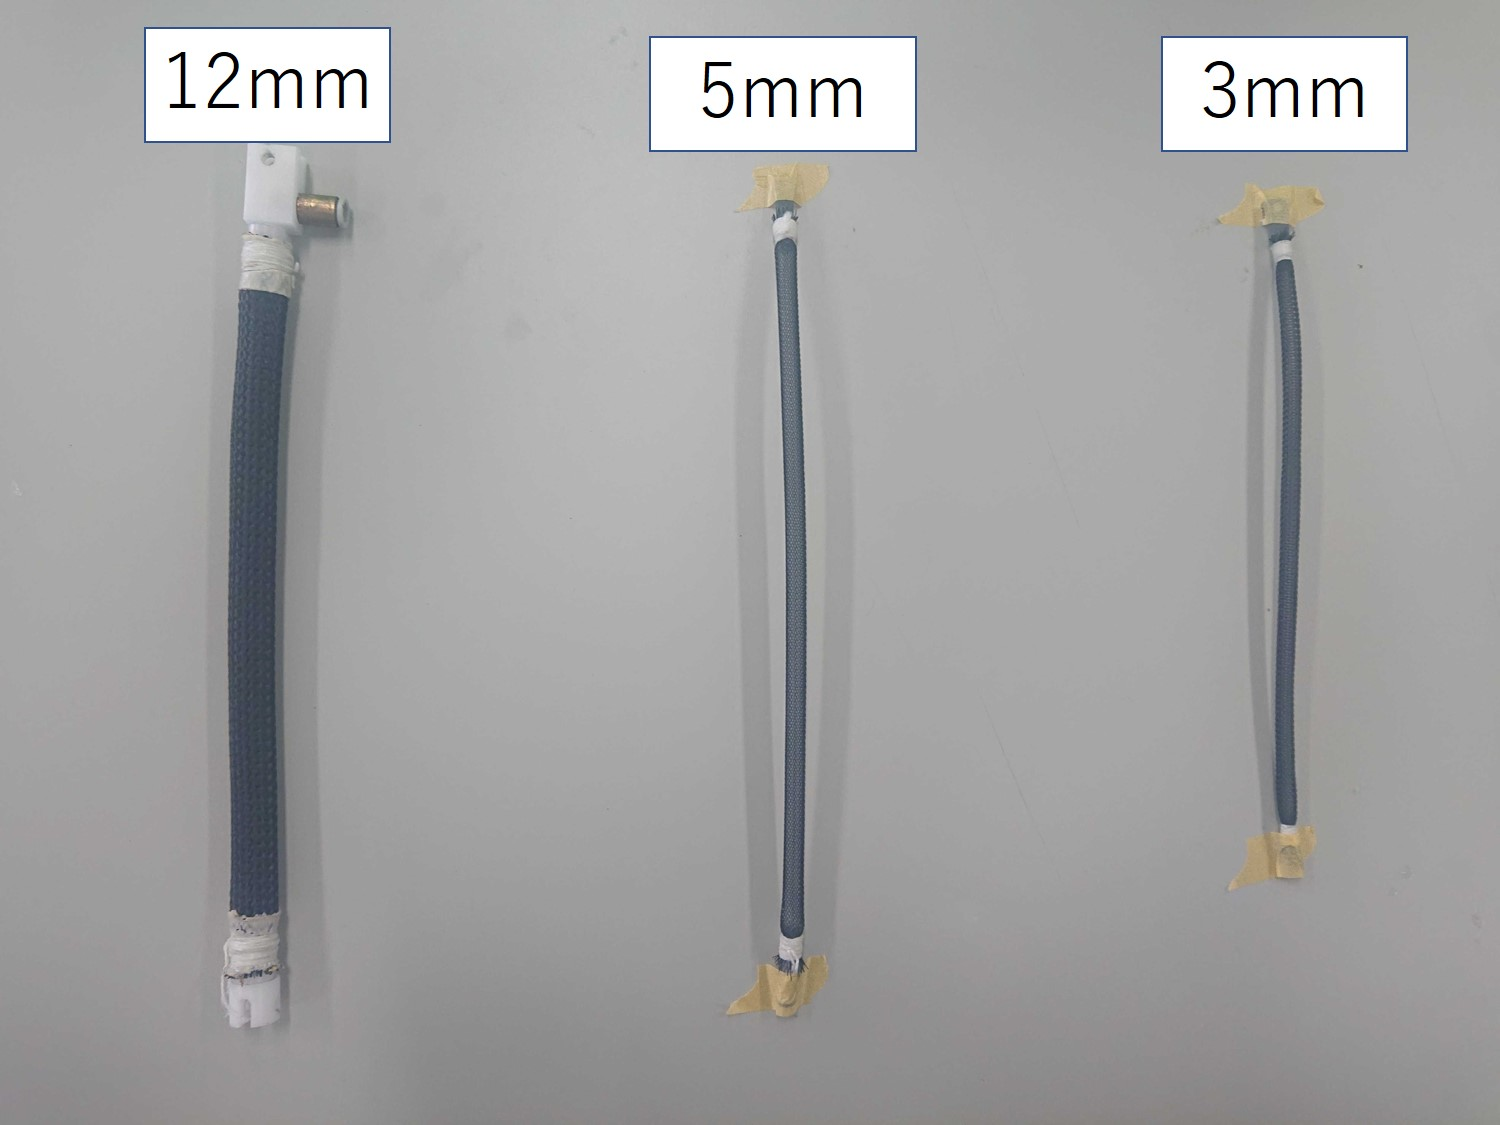
\includegraphics[scale=0.15]{mpa.JPG}
    \vspace{-6.5mm}
    \caption{MPAの外径}
    \label{fig:MPA}
  \end{minipage}
  \hspace{0.04\columnwidth}
  \begin{minipage}[b]{0.47\columnwidth}
    \centering
    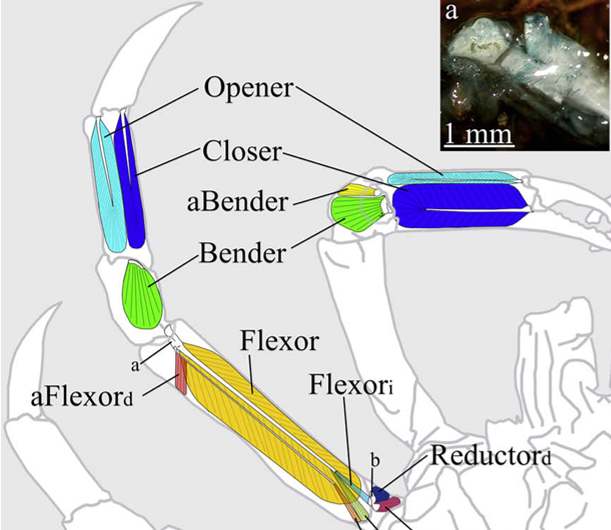
\includegraphics[scale=0.26]{kani6.PNG}
    \vspace{-2mm}
    \caption{蟹の筋構造\cite{crab}}
    \label{fig:mus}
  \end{minipage}
\end{figure}
%%%%%%%%%%%%%%%%%%%%%%%%%%%%%%%%%%%%%%%%%%%%%%%%%%%%%%%%%%%%%%%%%%%%%%%%%%%%%%%

%%%%%%%%%%%%%%%%%%%%%%%%%%%%%%%%%%%%%%%%%%%%%%%%%%%%%%%%%%%%%%%%%%%%%%%%%%%%%%%
\begin{thebibliography}{99}

  \bibitem{wakimoto}
  脇本修一,
  細径McKibben型人工筋の開発と用途開拓,
  計測と制御,57巻,11号,pp.812-815,2018
  
  \bibitem{crabrobot}
  CHEN, Xi, et al. Study on the Design and Experimental Research on a Bionic Crab Robot with Amphibious Multi-Modal Movement, Journal of Marine Science and Engineering,10,12,p.1804,2022
  
  \bibitem{crab}
  Vidal-Gadea AG,Belanger JH, Muscular anatomy of the legs of the forward walking crab, Libinia emarginata (Decapoda, Brachyura, Majoidea), Arthropod Struct Dev, May;38(3),pp179-94, 2009
  
  % \bibitem{crab}
  % 佐藤武弘,自然科学のとびら,第17巻,1号,pp.7-8,2011
  
  
 \end{thebibliography}
 %%%%%%%%%%%%%%%%%%%%%%%%%%%%%%%%%%%%%%%%%%%%%%%%%%%%%%%%%%%%%%%%%%%%%%%%%%%%%%%
\end{document}